% Metoddelen redogör för vad du gjort och hur du gått tillväga; det är
% en beskrivning av den metod som ligger till grund för det du kommit
% fram till och hävdar i din rapport.

% Beskrivningen i metoddelen ska vara koncis snarare än helt
% uttömmande men ska samtidigt göra det möjligt att upprepa studien

% Metoddelen ska inte vara en omgjord labbinstruktion och den ska inte
% heller innehålla teori med mindre än att teoretiska hänsyn har haft
% en direkt inverkan på metoden.

% Metoddelen skrivs nästan alltid i dåtid (imperfekt) och ofta används
% passiv form för att beskriva forskningsaktiviteter.

\chapter{Metod/Genomförande: Beskrivning av konstruktionen av läromaterialet}

% TODO: Är det intressant att ha med HUR vi, genom research, kom fram
% till att göra en specifik sak och varför den är bra?
%
% E.g. "Genom att läsa i bok A om område B så kom vi fram till att vi
% ska applicera metod C för att lösa problem D. Enligt bok A är metod
% C bra därför att ..."
% vs.
% "Vi valde att lösa problem D genom att applicera metod C. Metod C är
% bra därför att ...[ev. källhänvisning]."

TODO: Nånting om hur processen såg ut, lite mer meta. I.e. hur
arbetade vi i allmänhet? Scrum, vattenfall? Med issue-tracker, med
jira? Versionshantering? Etc.

\begin{draft}

Läromaterialet består av ett antal kapitel som vardera behandlar ett fysikaliskt område. Skapandet av läromaterialet har skett \textit{kapitelvis}. För varje kapitel har en process följts. Denna process illustreras i figur \ref{fig:hejhejhej}.

  \begin{figure}[h]
    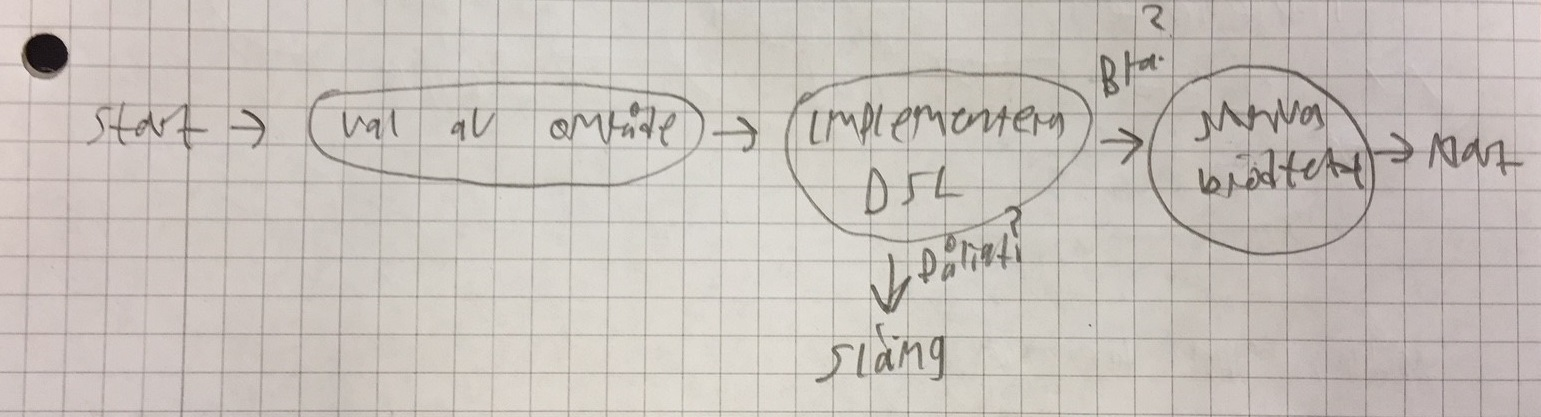
\includegraphics[width=\linewidth]{figure/hejhejhej.jpg}
    \caption{Översikt över processen med att skapa kapitlena i läromaterialet.}
    \label{fig:hejhejhej}
  \end{figure}

Som figur \ref{fig:hejhejhej} visar så bestod processen med att skapa ett kapitel av tre steg. Det första steget var att välja ett fysikaliskt område att behandla. Den andra steget var att implemenetera ett DSL för området. Det tredje steget var att skriva förklarande brödtext till det området.

Figuren visar också att, beroende på utfallet i implementationssteget, så antingen skrotas ett område eller gås vidare med. Huruvida området är lämpligt diskuteras i <ett diskussionskapitel>.

Läromaterialet publicerades i slutändan på en tillhörnade hemsida.

Resten av detta kapitel behandlar de olika stegen i den kapitelvisa processen mer i detalj. Det behandlar också publicering på hemsidan i närmare detalj.


\end{draft}

TODO: Sektion om våra litteraturstudier? Känns lite skumt att ha,
men 2016 hade. Litteratur är väl bara intressant att ha med som
refens när man refererar till fakta eller motiverar ett val? Själva
studieprocessen, i.e. HUR man nådde beslutet, är väl inte alls lika
intressant att ha med som VARFÖR man tog beslutet?

\begin{binge}
\section{Selektion av arbetsområden}

TODO: Hur hjälpte det senare Åke mötet? Med vad?

\begin{draft}

De områden som behandlas i läromaterialet kan klassificieras som antingen \textit{grundläggande} eller \textit{komposita}. Ett grundläggande område är ett område som inte bygger på något tidigare område. Ett exempel är vektorer. Ett komposit område är ett område som bygger på andra områden. Ett exempel är lutande plan, som använder sig av vektorer.

\subsection{Grundläggande områden}

  Först kontaktades Åke Fäldt, som är examinator för kursen TIF085,
  Fysik för Ingenjörer. Åke befrågades om vilka områden han tycker att
  studenter verkar ha svårt för, och svarade att studenter i allmänhet
  verkar ha svårt för att sätta upp egna, mentala modeller för många
  problem och koncept. ``Man tar genvägar (som ofta är fel) och bygger
  inte från det som man är säker på gäller'' skrev han, och han pekade
  ut infinitesimalkalkyl som ett speciellt svårt område:
  ``Infinitesimalkalkyl är ju en av hörnpelarna i fysiken och
  studenterna har trots att de har läst ganska mycket matematik
  jättesvårt att använda detta på verkliga system''.

  För att identifiera mer specifika ämnesområden att arbeta med,
  studerades kursboken *Univeristy Physics*. Speciellt av intresse var
  kapitel som berörde saker som Åke Fäldt tidigare pekat ut som svåra,
  och kapitel som använde sig av specifik syntax. Domänspecifik syntax
  var av intresse att finna, då en betydlig del av domänspecifika språk
  är modellering av just syntaxen. Även områden som projektgruppen fann
  personligen intressanta, och områden som inte var av direkt intresse,
  men som utgjorde en kritisk beståndsdel av mer intressanta områden,
  valdes ut.

  De valda grundområdena definierades sådana att de var fristående, i
  så god mån som möjligt, för att kunna arbetas med parallellt. De
  områden som valdes ut blev: Vektorer, Enheter, och Matematisk
  analys.

  Vektorer eftersom det är en viktig grundsten i mekanik. Alla krafter,
  hastigheter, och accelerationer, betraktas oftast som vektorer i
  planet eller rymden, och dessa är alla fundamental element i
  mekanik.

  Enheter eftersom det är viktigt för studenter att förstå sig på hur
  dimensioner påverkas av algebraiska operationer. Det kan också vara
  hjälpsamt att kunna utföra automatisk, datorassisterad
  dimensionsanalys på ens beräkningar.

  Analys eftersom alla koncept i klassisk mekanik är relaterade genom
  matematisk analys. Mer specifikt används differenser för att beskriva
  medelrörelse, och infinitesimalkalkyl för att beskriva
  momentanrörelser. Vidare var infinitesimalkalkyl just det område som
  Åke Fäldt pekade ut som speciellt viktigt, och något som studenter har
  svårt för.

  \begin{binge}
  
  \subsection{Komosita områden}
  
    När en mängd av de fristående, grundläggande områdena var
    fädigimplementerade så formulerades mer tillämpade områden i form
    av problemmängder. De tillämpade fysikproblemen krävde ofta bruk
    av flera olika DSL för att lösa. Exempelvis kan ett rörelseproblem
    använda sig av både differentialkalkyl och dimensionsanalys.  Till
    dessa områden skrevs därför komposita DSL som kombinerade en mängd
    grundläggande DSL för att bättre kunna beskriva problemdomänen.

    De tillämpade områdena var inte lika lätthanterliga som de
    grundläggande områdena. Det var sällan uppenbart hur komposita DSL
    skulle skrivas och appliceras, och vissa områden visade sig vara
    olämpade att skriva DSL för. Vidare motivation av varför vissa
    områden var mindre lämpade för den sortens DSL som skrevs finnes
    under Diskussionskapitlet. (TODO: Fast en kort motivation här med
    kanske?). Detta medförde att experimentering med DSL
    implementation var ett viktigt steg i processen att selektera lämpliga
    tillämpade områden, då experimenteringen kunde visa hurvida ett område
    var lämpat att skriva DSL för eller inte. TODO: oj vad hände med
    denna meningen, jag är trött.
  \end{binge}

  De komposita områden som valdes ut blev: Momentan- och
  medel-rörelse, TODO: Mer, etc.

  Momentan- och medel-rörelse eftersom de direkt utgör en stor delmängd
  av alla problem inom mekanik på den aktuella nivån. Väldigt många av
  de uppgifter studenter lär sig lösa inom mekanik är
  sträcka/hastighet/acceleration/kraft problem. Hur lång tid tar det att åka en
  sträcka om man har en viss medelhastighet? Om ett objekt med massa $m$
  påverkas av en kraft som varierar enligt $sin(t)$, vad är då
  momentanhastigheten vid $t=10$?
\end{draft}

TODO: Nåt om hur områdesvalen speglas i strukturen av läromaterialet?

\end{binge}

\begin{binge}
  \section{Implementation av DSL för områdena}

  \begin{draft}
    Det första steget vid implementering av ett DSL var alltid
    experimentering. Det finns ingen absolut, kanonisk metod att skriva
    ett DSL på, speciellt för specifik fysik, så experimentering var
    viktigt för att finna lämpliga representationer av syntax och andra
    element av DSL.
  \end{draft}

  TODO: Förbättra

  \subsection{Implementation av }

  \begin{draft}
    Av de områden som selekterats för projektet, valde varje gruppmedlem
    varsitt område att arbeta med. Från experimentering fanns syntaxträd
    och funktioner som väl kunde representerade matematiken och andra
    koncept inom området. Kraven för vad som ansågs som en bra
    representation var i huvudsak baserade på intuitionen hos
    gruppmedlemmarna som erfarna haskell-programmerare, och i viss mån
    individuellt definierade för varje gruppmedlem. I praktiken var de
    slutgiltiga implementationerna oftast också de minsta
    implementationerna, med avseende på bl.a. antal kodrader.

    TODO: Stycket om ``vår intuition som erfarna haskell-programmerare''
    lät lite pretentiöst. Annat ordval? ``vår intuition som studenter
    som läst DSLsofMath kursen"?''

    Alla områden krävde i varierande mån inläsning och studering av
    Haskell, Agda, fysik, matematik, och DSL. Till exempel krävde
    enhets-DSLet inläsning om ett gäng Haskell-extensions och
    typnivå-programmering. För att kunna bevisa korrekthet i beteende
    för vissa DSL studerades även Agda.

    I allmänhet implementerades DSL i Haskell som en kombination av
    syntaxträd, funktioner för att manipulera dessa träd, och
    evalueringsfunktioner till någon slags semantisk domän. Komposita
    DSL var istället mer TODO: beskrivning. Varje DSL, grundläggande och
    komposit, parades även ihop med en mängd fysikproblem att appliceras
    på, sådant att läsaren ska få förståelse för hur DSLen kan brukas
    utöver hur de implementeras.

    TODO: Vi bevisade/försökte bevisa grejer med. Skriv om att DSL i
    allmänhet hade bevis eller tester för att verifiera korrekthet.
  \end{draft}

  Syntax analyserades och modellerades i syntaxträd. För vissa områden
  (enheter?) definierades även ett semantiskt värde som representerade
  en slags kanonisk form.

  För vektorer gjordes ...

  För enheter gjordes ...

  För analys gjordes ...

  För annat gjordes ...

  \subsection{Komposita områden}

  Importera DSLerna för varandra för att göra mer komplicerade grejer.

  Eller, \emph{Bruk av de mer fundamentala/teoretiska DSLerna för att
    angripa områden av mer ``tillämpad'' natur (såsom Krafter, Arbete,
    etc) )}(?)

  !! Områden/moduler soom bygger vidare på redan implementerade områden.

  stack, git kan säkert passa här för att beskriva hur vi samarbetade
  med sammanfogningen.

\end{binge}

\begin{binge}
  \section{Skriva lärotext}

  En massa bra och fina didaktiska metoder användes för att skriva
  riktigt fin lärotext. Texten skrevs i LHS format, vilket innebar att
  beskrivande text alltid finns i samband med koden den har att göra
  med.

  TODO: Referera till Donald knuth och literate programming. Literate
  programming som ``paradigm'' känns relevant för hur vi skriver
  lärotext.

  TODO: Motivera varför vi valde LHS

  TODO: Motivera varför vi valde hemsida istället för PDF.

  TODO: Motivera varför vi valde Markdown istället för LaTeX i LHS
  filerna.

  \subsection{Didaktik/språk/utlärningsmetod}

  Lättsamt språk o en gnutta humor för att hålla kvar
  uppmärksamhet. Relaterat till Attention i ARCS modellen (2016
  använde den. Såg vettig ut).

  TODO: Expandera. Vad exakt använder vi för didaktisk metod? Samma
  som appliceras i Learn You a Haskell, mer eller mindre. Fånga
  uppmärksamhet med lite humor och lättsamhet etc.

  \subsection{Skriva lärotext till DSL}

  När en modul DSL var färdigimplementerad, ofta med nödtorftiga
  kodkommentarer, skrevs brödtext som förklarade kod-delen. Detta
  efterföljande steg för att förstå koden är viktigt, och är ett krav
  för att man ska kunna skriva en förklaring (och förstå den) om
  kopplingen till fysik.

  Vidare skrevs brödtexten som sammankopplade DSL och fysik. När
  själva koden var på plats skrevs hur den relaterar till och
  modellera fysik. I slutändan skrevs också inledning och avslutning
  till kapitlet.

  \subsection{Skriva läromaterial för hur DSL appliceras för problemlösning}

  Vari vi visar att DSLerna både är praktiskt användbara, likt Wolfram
  Alpha, och att implementationen+applikationen hjälper oss förstå
  mekanik i allmänhet och probleminstanserna i synnerhet.
\end{binge}

\begin{binge}
  \section{Sammanställning, presentation, och publicering}

  Läromaterialet publiceras på en internethemsida, varpå man kan läsa
  allt o ha skoj.

  \subsection{Beskrivning}

  Ett build-script hämtar .lhs källfilerna, i vilka brödtexten är
  skriven med markdown. Rendrar med pandoc, och sätter in lite
  navigationselement etc. med hjälp av eget templating-system. Manuellt
  läggs sedan stoffet på gh-pages branchen för att automatiskt visas på
  dslsofmath.github.io/BScProj2018.

  Obs: Medan bygget är scriptat så är inte publiceringen det, och
  ingenting genereras/publiceras automatiskt kontinuerligt. Måste köra
  scriptet manuellt och lägga stoff på gh-pages branchen.

  \subsection{Build-script}

  I.e. implementation av python-build-scriptet i mer detalj.

  TODO: Är detta ens intressant? Viktigt för att producera sidan såklart, men
  inte intressant ur varken matte eller haskell/DSL perspektiv.

  \subsection{Hemsidan}

  Nåt om design, läslighet, grafik(?), navigation, avsiktligt undvikande
  av javascript, etc.

  Tänker lite samma med denna sektion som ovan. Har ju ingenting med
  varken matte eller DSL att göra i sig, så kanske inte så intressant?
  Samtidigt är det kanske lite intressant ur pedagogik-aspekten. Kan det
  kanske vara lättare/roligare att lära sig om sidan är fin och
  lättläst? Att javascript inte krävs gör att sidan kan visas ordentligt
  även om man sitter i U-land med dålig/gammal/billig telefon.
\end{binge}

\begin{binge}
  \section{Test och återkoppling}

  % Återkoppling från examinator (NAD): "Nils Anders Danielsson <nad@cse.gu.se>
  % 27 Feb (1 day ago)
  % to Patrik, Andreas
  % Hi,Your BSc project groups both try to make tools for learning. I had some
  % discussion with Andreas' group about their plans for evaluating how well
  % their product works. My position is that, given the resource limits of
  % these projects (and general problems of reproducibility in social
  % sciences), it is very hard to perform an evaluation that gives useful
  % results. I don't mind if your groups try to perform some kind of
  % evaluation, but I suggest that you tell them to avoid overstating the
  % importance of the evaluations in the final reports."
  % Jag tror det är kompatibelt med det jag sagt tidigare - att göra en "ordentlig" utvärdering av det pedagogiska utfallet är komplicerat och tar (kalender-)tid.
  % Informell utvärdering av en testgrupp bör dock ingå.

  Test på försöksstudenter. Återkoppling med Åke(?).

  Nog bra att vara explicit här med att det inte är en rigorös empirisk
  studio, om inte det redan täckts väl i Avgränsningar.

\end{binge}